\section{System}
\label{sec:system}

When the position of a particle is chosen to be the global best, its personal best is updated as well.
In this case, $ x(k) = x^{P}(k) = x^{G}(k) $, which means this particle will not move till a new global best is found.
We could view this particle as a leader of this swarm.
The topology is given in Figure \ref{fig:leader_follower}.

\begin{figure}[tbph]
\centering
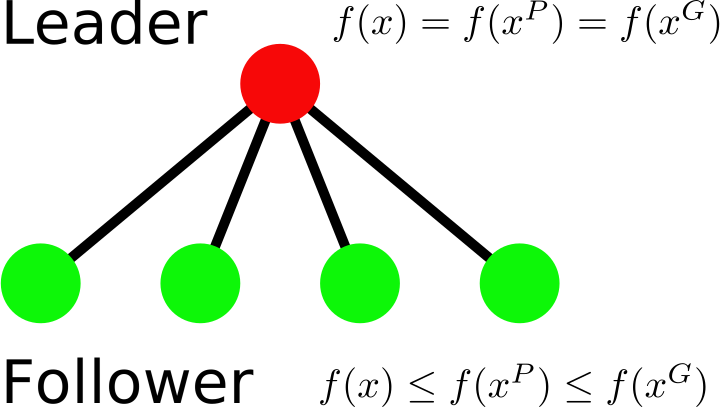
\includegraphics[width=0.5\linewidth]{./fig/leader_follower}
\caption{}
\label{fig:leader_follower}
\end{figure}


The optimal search process of the swarm becomes a leader competition among the particles.
Once a particle finds a new global best, it becomes the leader of the swarm.
The other particles are the followers, which are attracted to the leader by the impact of the global best.
By Property \ref{prop:unconverge_neq_gb}, we know that a particle will never stop moving if the personal best and the global best are inconsistent.
Thus, we can view the movements of the followers are sampling in the solution space to solve the inconsistency between its own personal best and the global best.




